\subsection{Comparação entre Controlador Proporcional, PID com Dados Iniciais e PID Ajustado}
Esta seção apresenta uma análise comparativa do desempenho de três configurações distintas de controladores: Proporcional, PID com valores iniciais e PID ajustado. A análise foca na resposta dos controladores em termos de estabilidade, tempo de resposta e precisão no estado estacionário. Ajustar o parâmetro \(K_p\) tem implicações significativas na dinâmica de controle, impactando diretamente a eficácia e eficiência do sistema.

\begin{figure}[H]
    \centering
    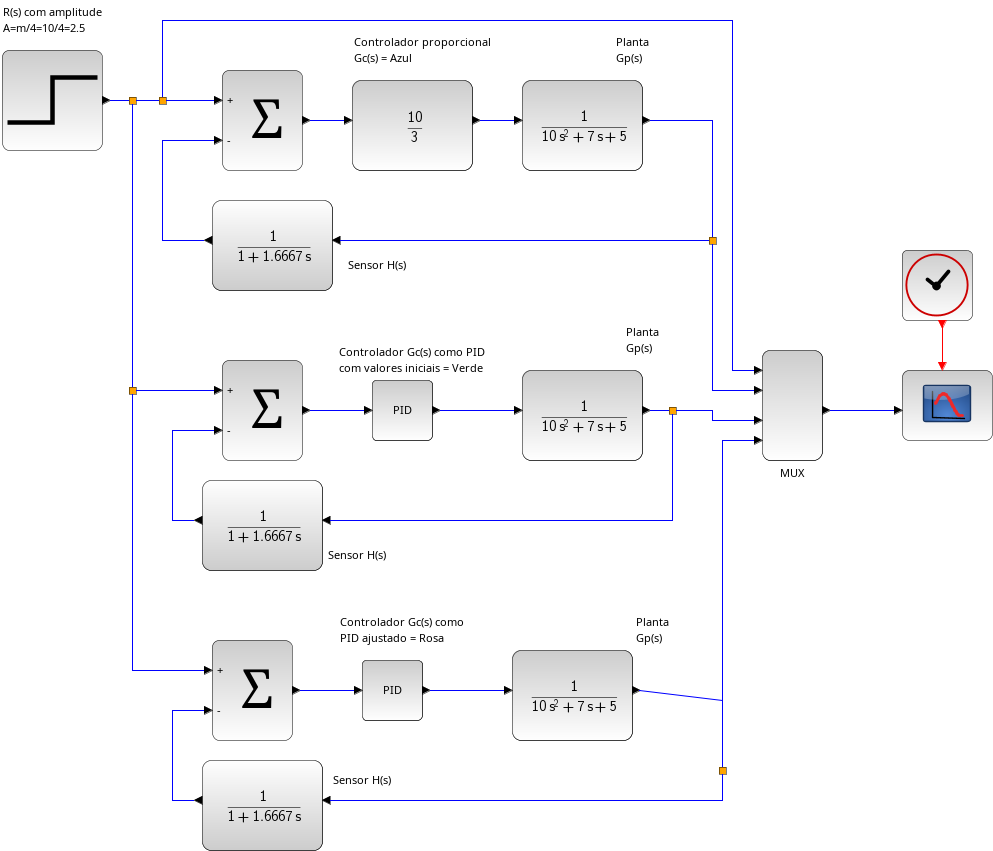
\includegraphics[width=0.8\textwidth]{6-atividade/assets/d/diagrama-comparacao-proporcional-pid-pid-ajustado.png}
    \caption{Diagrama de resposta do sistema com diferentes configurações de \(K_p\).}
    \label{fig:diagrama-comparacao-proporcional-pid-pid-ajustado}
\end{figure}

\begin{figure}[H]
    \centering
    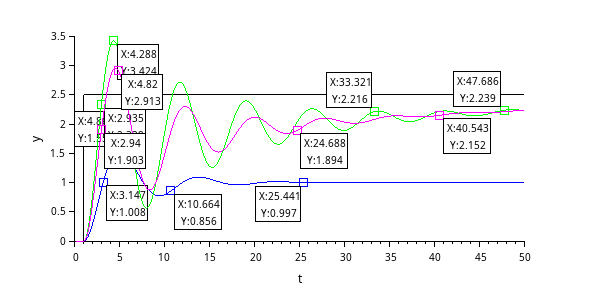
\includegraphics[width=0.8\textwidth]{6-atividade/assets/d/comparacao-proporcional-pid-pid-ajustado.png}
    \caption{Comparação das respostas temporais dos controladores sob a mesma condição de teste.}
    \label{fig:comparacao-proporcional-pid-pid-ajustado}
\end{figure}


\subsubsection{Análise dos Controladores}

\subsubsection{Controlador Proporcional (Cor Azul)}
\textbf{Comportamento:} O controlador proporcional, adequado para sistemas onde precisão extrema não é primordial, mostra uma resposta rápida inicial, mas falha em eliminar o erro de estado estacionário, uma limitação comum devido à ausência de ação integral.
\textbf{Estado Estacionário:} A resposta estabiliza significativamente abaixo do valor de referência, evidenciando a limitação deste tipo de controlador em corrigir completamente o erro de estado estacionário, adequado para aplicações onde desvios menores são toleráveis.

\subsubsection{PID com Valores Iniciais (Cor Verde)}
\textbf{Comportamento:} Este controlador exibe um overshoot inicial significativo e oscilações antes de estabilizar, característica de uma resposta rápida seguida de uma correção intensa pela ação integral.
\textbf{Estado Estacionário:} Atinge e mantém o valor desejado, com a componente integral ajustando o erro acumulado e garantindo que a saída final corresponda exatamente ao valor de referência.

\subsubsection{PID Ajustado (Cor Rosa)}
\textbf{Comportamento:} A redução de \(K_p\) para 7.1664 atenuou o overshoot e proporcionou uma abordagem mais suave na resposta ao degrau, indicando um melhor equilíbrio entre as ações proporcional e integral.
\textbf{Estado Estacionário:} Alcança o estado estacionário com menos oscilações, refletindo uma melhoria na estabilidade geral do sistema. A ação integral continua a compensar qualquer erro residual, assegurando que a saída esteja alinhada ao valor do degrau.

\subsection{Conclusão e Implicações para o Ajuste de \(K_p\)}
A redução de \(K_p\) para 80\% do valor inicial demonstrou melhorar a resposta do sistema ao reduzir o overshoot e aumentar a estabilidade sem comprometer excessivamente a resposta rápida. Essa modificação evidencia a necessidade de um equilíbrio cuidadoso na configuração de \(K_p\), onde a eficiência operacional e a estabilidade precisam ser otimizadas em conjunto.

\vspace{0.4cm}
\textbf{Considerações Adicionais:}
\begin{itemize}
    \item Uma redução adicional de \(K_p\) pode ser explorada para sistemas onde a estabilidade é mais crítica que a resposta rápida. No entanto, é essencial garantir que essa redução não comprometa a capacidade do sistema de responder a perturbações repentinas.
    \item O ajuste fino de \(K_p\) deve ser realizado com consideração das características específicas do sistema e das condições operacionais. A simulação controlada é recomendada para determinar o melhor conjunto de parâmetros, equilibrando estabilidade e precisão.
\end{itemize}

Embora a configuração atual de \(K_p\) tenha mostrado resultados promissores, é fundamental reconhecer que sempre existem oportunidades para refinar ainda mais os parâmetros do controlador PID. O processo de ajuste manual de \(K_p\), \(K_i\), e \(K_d\) deve ser contínuo e iterativo, adaptando-se às mudanças nas condições operacionais e às necessidades específicas de cada sistema. Ajustes manuais são essenciais para calibrar o controlador de modo a responder adequadamente sob diferentes cenários, permitindo uma melhoria contínua do desempenho do sistema.
